\documentclass[xcolor=dvipsnames, 14pt]{beamer}

\usepackage{beamerthemesplit}
\usepackage[mathscr]{eucal}
\usepackage{pgfpages}
\usepackage{graphicx}
\graphicspath{ {c:/Users/Marissa/} }
\usepackage{array}
\usepackage{comment}
\usepackage{hyperref}
\usepackage{import}
\usepackage{amsmath, amsfonts, amscd, amssymb}
\usepackage{epsfig}
\usepackage{graphicx}
\usepackage{url}
\usepackage{mathrsfs}
\usepackage{makeidx}
\usepackage{color}
\usepackage{verbatim}
\usepackage{listings}
\usepackage{multicol}
\usepackage{algorithmicx}
\usepackage[plain]{algorithm}
\usepackage[noend]{algpseudocode}
\usepackage{float}
\usepackage{paralist}
\usepackage{caption}
\usepackage{subcaption}
\usepackage{textcomp}
\usepackage[framemethod=tikz]{mdframed}
\usepackage{tikz}
\usetikzlibrary{arrows, automata, backgrounds, calendar, chains, decorations,
	matrix, mindmap, patterns, petri, positioning, shadows, shapes.geometric,
	shapes, trees}
\definecolor{boxbackground}{rgb}{1,0.976,0.882}

\usepackage{ulem}


\usepackage{setspace}
\usepackage{wrapfig}
\usepackage{float}
\usepackage{cancel}
\usepackage{multirow}
\newcolumntype{L}[1]{>{\raggedright\let\newline\\\arraybackslash\hspace{0pt}\vspace{0pt}}m{#1}}
\newcolumntype{C}[1]{>{\centering\let\newline\\\arraybackslash\hspace{0pt}}m{#1}}
\newcolumntype{R}[1]{>{\raggedleft\let\newline\\\arraybackslash\hspace{0pt}\vspace{0pt}}m{#1}}

\lstset{
language=Python,
basicstyle=\ttfamily\scriptsize,
keywordstyle=\color{blue}\ttfamily,
stringstyle=\color{red}\ttfamily,
commentstyle=\color{green!50!black}\ttfamily,
frame=single,
breaklines=true,
postbreak=\raisebox{0ex}[0ex][0ex]{\ensuremath{\color{violet}\hookrightarrow\space}},
backgroundcolor = \color{boxbackground},
showspaces=false,
showstringspaces=false,
}


\usepackage{mathtools}

\defbeamertemplate{section page}{mine}[1][]{
  \vspace*{\fill}
  \begin{centering}
    \begin{beamercolorbox}[sep=12pt,center]{part title}
      \usebeamerfont{section title}\insertsection\par
    \end{beamercolorbox}
  \end{centering}
  \vspace*{\fill}
}

\setbeamertemplate{section page}[mine]

\setbeamertemplate{footline}
{
  \leavevmode%
  \hbox{%
  \begin{beamercolorbox}[wd=.7\paperwidth,ht=2.25ex,dp=1ex,center]{author in head/foot}%
    \usebeamerfont{author in head/foot}{}
  \end{beamercolorbox}%
  \begin{beamercolorbox}[wd=.3\paperwidth,ht=2.25ex,dp=1ex,center]{title in head/foot}%
    \usebeamerfont{title in head/foot}{}
  \end{beamercolorbox}%
  }%
  \vskip0pt%
}



\usefonttheme[onlymath]{serif}
\usetheme{Madrid}
%Options: default, albatross, beaver, beetle, crane, dolphin, dove, fly, lily, orchid, rose, seagull, seahorse, whale, wolverine
%Crane is orange, fly is ugly, albatross is bad, dolphin ditches colorboxes, beaver is red on gray, beetle is gray background
%dove is straight up black on white, lily ditches colorboxes, whale is normal, seahorse is a light blue
\usecolortheme{seahorse}
\setbeamertemplate{navigation symbols}{} 
\setbeamertemplate{items}[square] 
\setbeamertemplate{table of contents}[square]
\setbeameroption{hide notes}


\title[]{A Computationally Driven Comparative Survey of Network Alignment, Graph Matching, and Network Comparison in Pattern Recognition and Systems Biology}
\author[M. Graham]{Marissa Graham \and \\Advisor: Dr. Emily Evans}
\institute{Brigham Young University}
\date{}

% it's a FORTY MINUTE PRESENTATION; budget like 10-15min for each blob, average like 12, few minutes for conclusion

% To discuss w/ Dr. Evans:
% What do I say first? 
% Have copy of PDF on ipad for scrolling and reference ok? Mostly for if I need to talk in detail about global alignment algorithms--need to remind myself
% How many pauses?

\begin{document}
\frame{\titlepage}

\begin{frame}{Motivation}
\begin{itemize}
\item Networks are a powerful way to model relationships between objects
\pause
\item How can we exploit this representation to gain insights about the objects being modeled?
\pause
\begin{itemize}
\item Visualization
\item Connectivity, paths, centralities, degree distributions, etc.
\item Comparison between networks
\end{itemize}
\end{itemize}
\end{frame}

\begin{frame}{Motivation}
\begin{itemize}
\item Two main fields of application for network comparison
\pause
\begin{itemize}
\item Pattern recognition (computer science)
\item Systems biology
\pause
\end{itemize}
\item Existing surveys are not truly interdisciplinary
\pause
\begin{itemize}
\item Lack of common terminology and background inhibits understanding
\item ``Reference dumping''
\item Difficult to determine most relevant works without prior expertise in a field
\pause
\end{itemize}
\item How can we create a more cohesive presentation?
\end{itemize}
\end{frame}

\begin{frame}{Approach}
\begin{itemize}
\item Curate a list of relevant papers
\begin{itemize}
\item First five pages of Google Scholar for ten different search terms
\pause
\end{itemize}
\item Construct a citation network from their reference lists
\pause
\begin{itemize}
\item Hand-format .txt file reference lists 
\item Look up metadata from freeform citation using the CrossRef REST API
\item Manually check unverified results and parse incorrect results
\end{itemize}
\end{itemize}
\end{frame}

\begin{frame}{The full citation network}
\centering
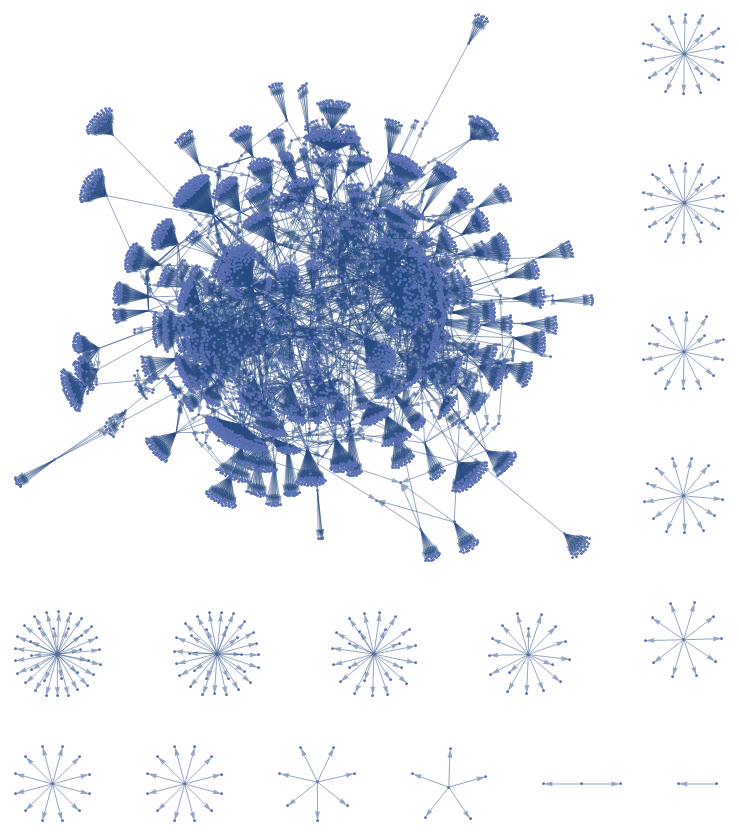
\includegraphics[width=0.7\textwidth]{full_citation_network.png}
\end{frame}

\begin{frame}{The pruned citation network}
\centering
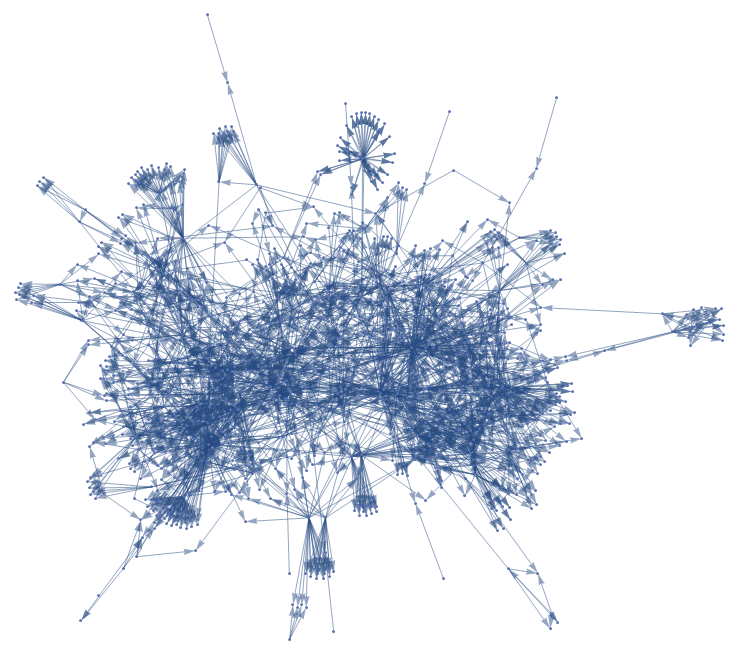
\includegraphics[width=0.7\textwidth]{subnetwork.png}
\end{frame}

\begin{frame}{Statistics}
\centering
\footnotesize
\begin{tabular}{| l | c | c | c | c | c | c |}
\hline
 & $G$ & $G_p$ & sciMet & zewail & $R$ & $R_d$ \\ \hline\hline
Vertices & 5793 & 1062 & 1092 & 3145 & 5793 & 5793 \\ \hline
Edges & 7491 & 2775 & 1308 & 3743 & 7491 & 7491\\ \hline 
Mean degree & 1.29 & 2.61 & 1.20 & 1.19 & 1.29 & 1.29 \\ \hline 
Fraction with children & 0.038 & 0.193 & 0.523 & 0.599 & 0.733 & 0.038 \\ \hline 
Diameter & 10 & 9 & 14 & 22 & 21 & 9\\ \hline 
Connected components & 16 & 1 & 114 & 281 & 504 & 3 \\ \hline 
\% in giant component & 96 & 100 & 78.4 & 79.7 & 90 & 99.9 \\ \hline 
\end{tabular}
\end{frame}

\begin{frame}{SciMet and Zewail (for reference)}
\centering
\begin{minipage}{0.47\linewidth}
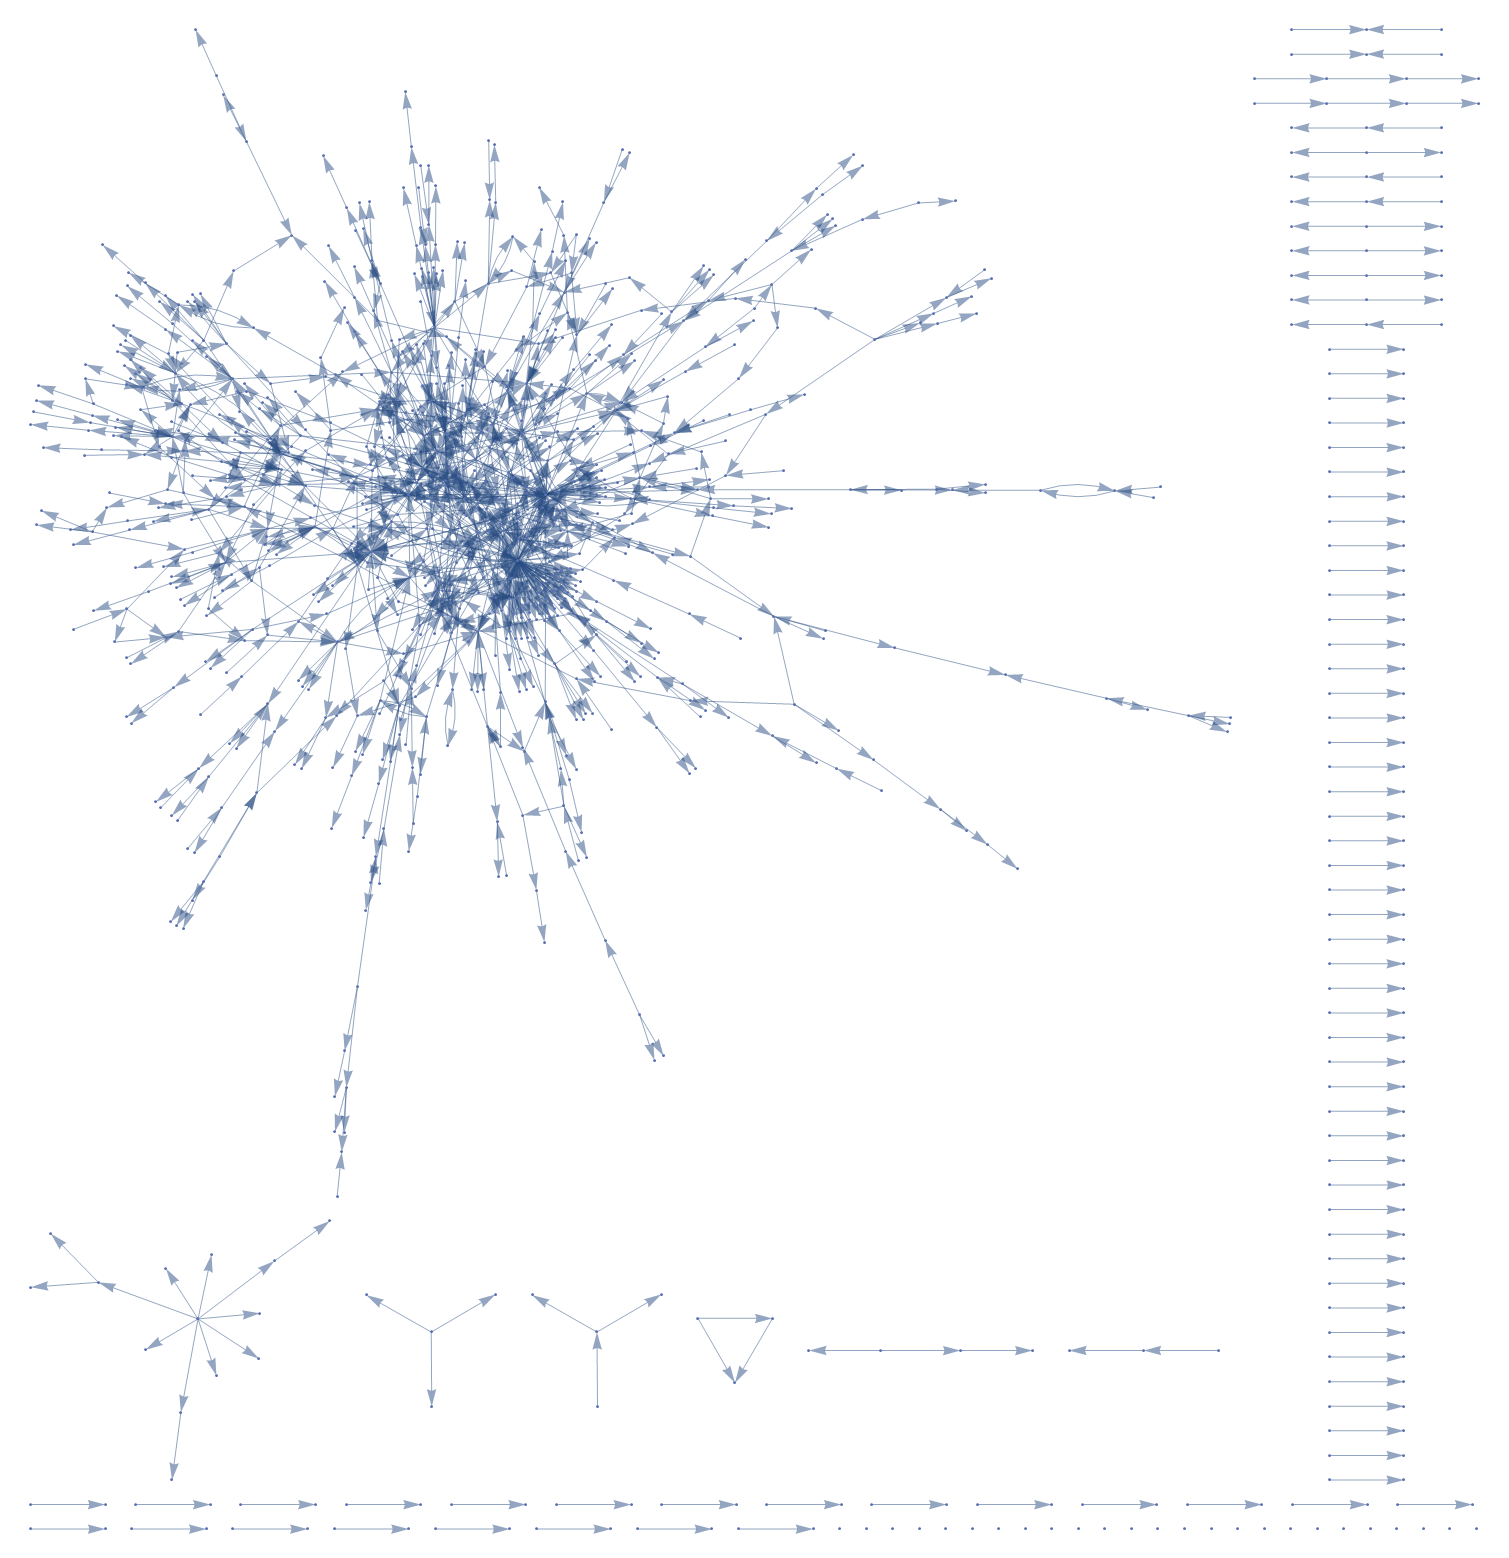
\includegraphics[width=\textwidth]{display_sciMet.png}
\end{minipage}\hfill
\begin{minipage}{0.47\linewidth}
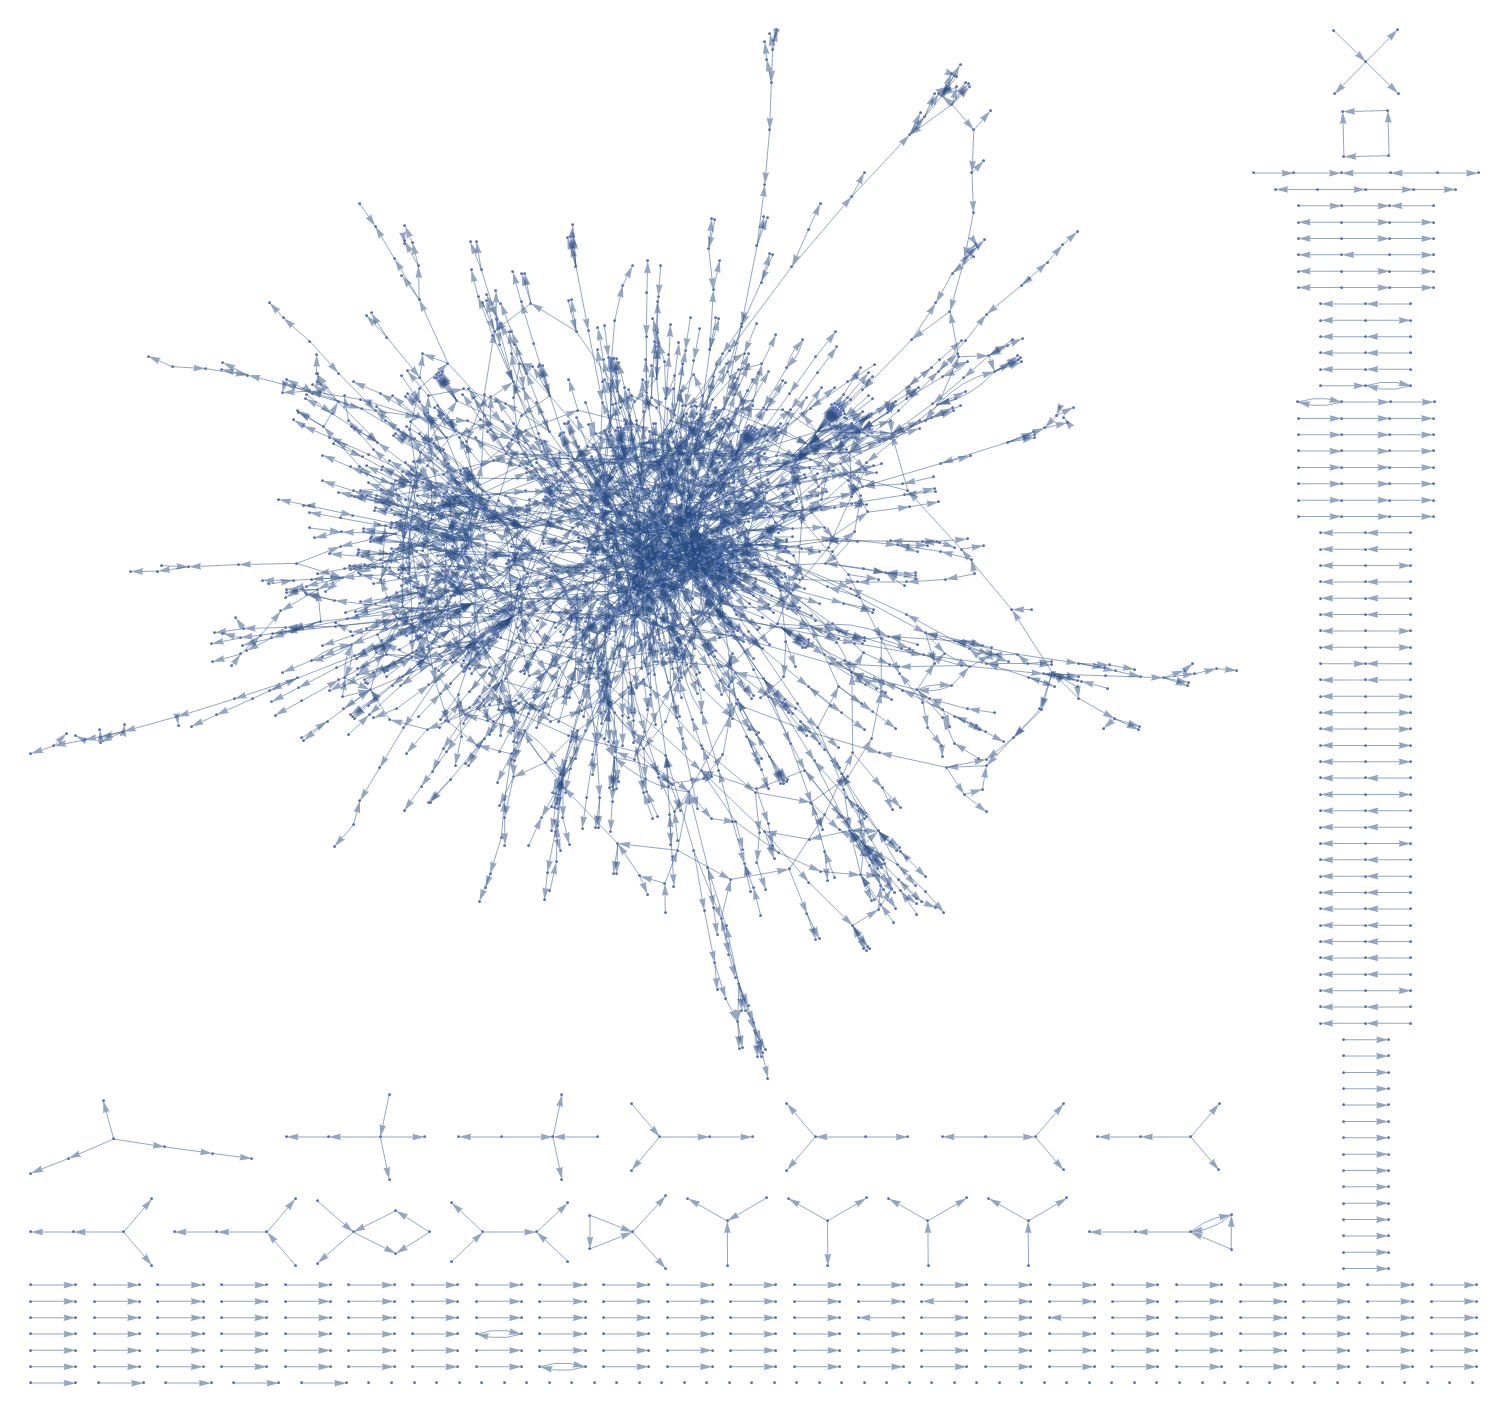
\includegraphics[width=\textwidth]{display_zewail.png}
\end{minipage}
\end{frame}

\begin{frame}{Centrality}
\centering
\begin{minipage}{0.45\linewidth}
\begin{itemize}
\item Indegree
\item Outdegree
\item Betweenness
\item Closeness
\item HITS authority
\item HITS hub
\end{itemize}
\end{minipage}\hfill
\begin{minipage}{0.45\linewidth}
\centering
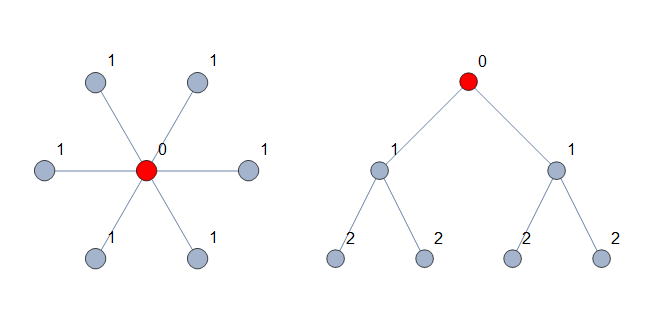
\includegraphics[width=\textwidth]{closeness_demo.png}
\scriptsize Closeness
\end{minipage}
\end{frame}

\begin{frame}{Centrality}
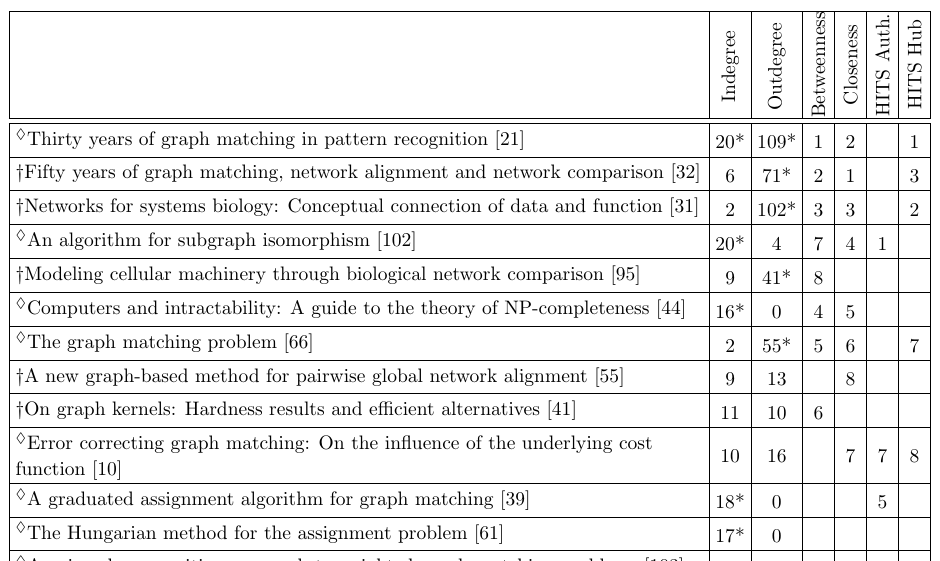
\includegraphics[width=\textwidth]{giant_table_ex.png}
\end{frame}

\begin{frame}{Partitioning}
\centering
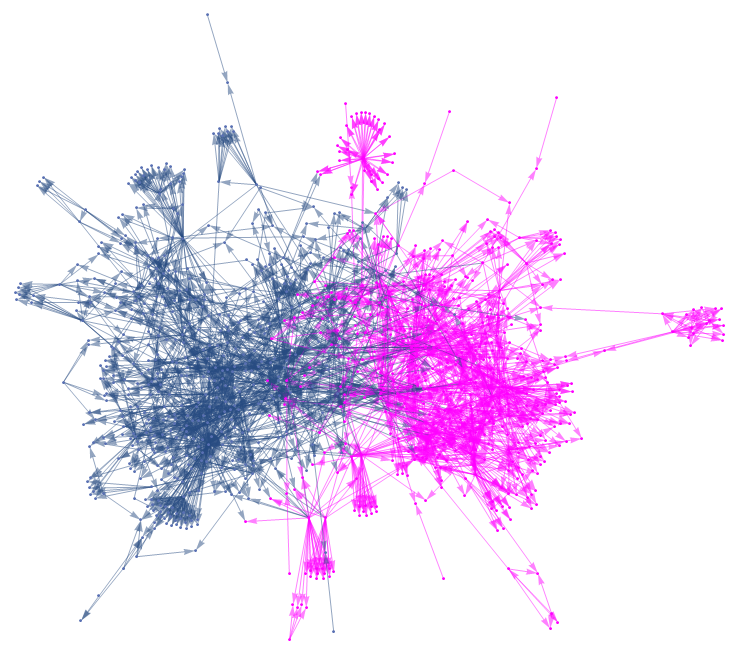
\includegraphics[width=0.7\textwidth]{subnetwork_partition.png}
\end{frame}

\begin{frame}{Partitioning}
\begin{itemize}
\item Do the ``clumps'' seen match our observations about the two main fields of application?
\pause
\item Subject information not available in metadata
\pause
\item Tag papers using journal titles (which are available)
\begin{itemize}
\item Ex) ``biology'', ``cell'', ``protein'', ``DNA'' 
\item Ex) ``computer vision'', ``ACM'', ``IEEE'', ``software''
\pause
\item Gives us results for 54\% of papers in the pruned network
\end{itemize}
\end{itemize}
\end{frame}

\begin{frame}{Partitioning}
\centering
\begin{minipage}{0.55\linewidth}
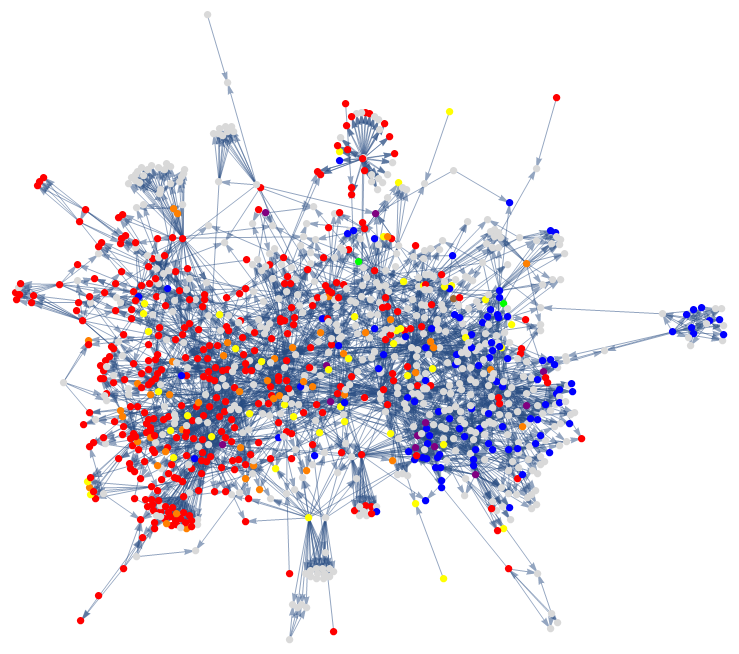
\includegraphics[width=0.9\textwidth]{color_coded_full.png}
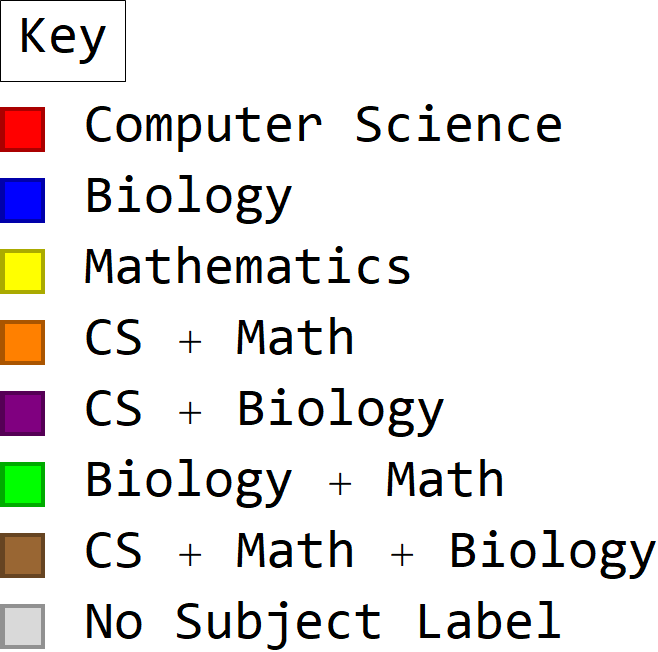
\includegraphics[width=0.3\textwidth]{color_key.png}
\end{minipage}\hfill
\begin{minipage}{0.4\linewidth}
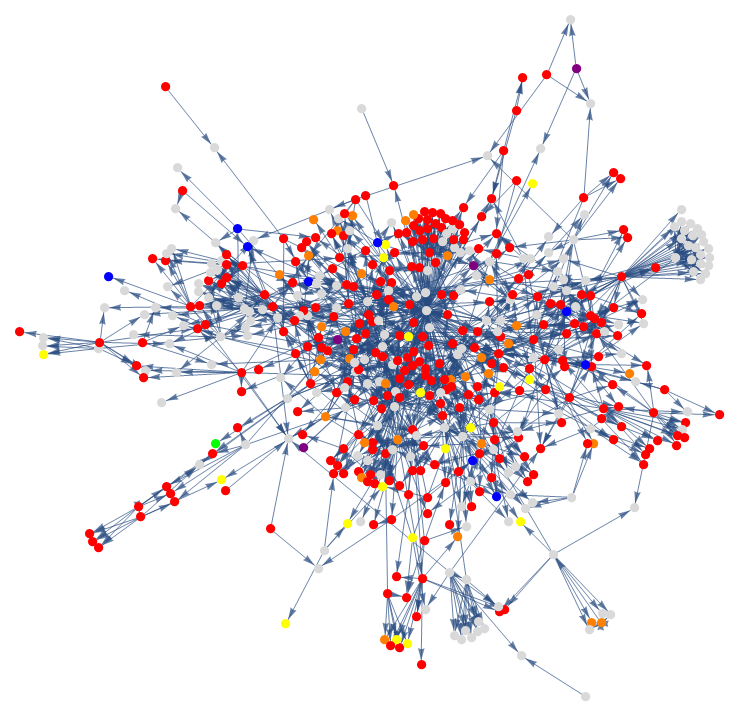
\includegraphics[width=0.8\textwidth]{color_coded_left.png}
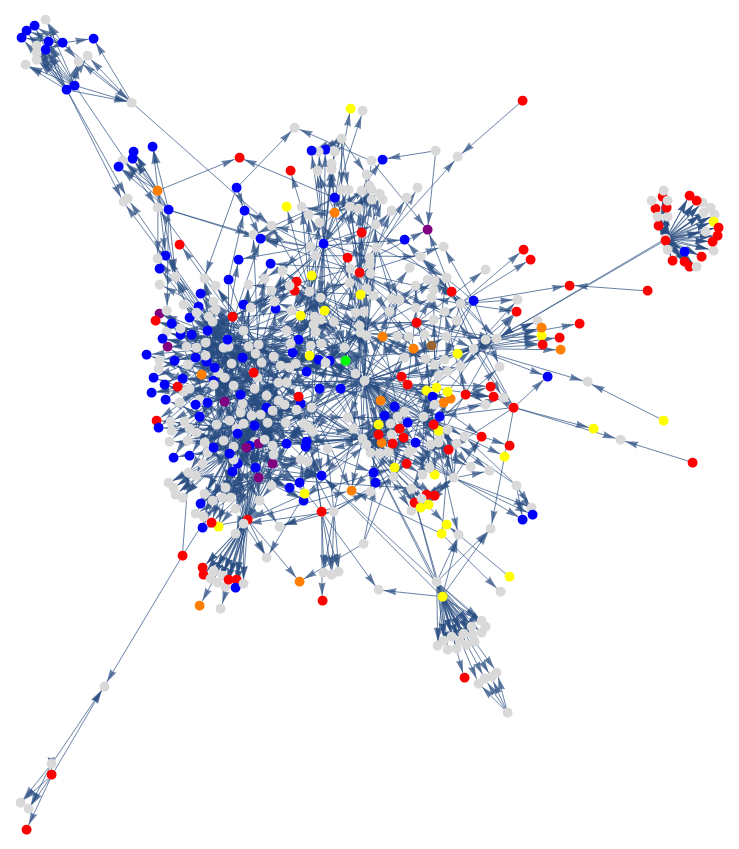
\includegraphics[width=0.8\textwidth]{color_coded_right.png}
\end{minipage}
\end{frame}

\begin{frame}{Assortativity}
\centering
\footnotesize
\begin{tabular}{|l|r|r|}
\hline
 & $G$ & $G_p$ \\ \hline\hline
Outdegree & -0.0178 & -0.0141 \\ \hline
Publication year & 0.0067 & 0.0041 \\ \hline
Citation count & 0.0006 & 0.0654 \\ \hline
Reference count & 0.0193 & -0.0061 \\ \hline
Tagged with any subject & 0.1089 & -0.0094 \\ \hline
Subject & 0.1837 & 0.0712 \\ \hline
Subject is CS & 0.2624 & 0.1529 \\ \hline
Subject is biology & 0.3354 & 0.1773 \\ \hline
Subject is math & 0.0732 & 0.0164 \\ \hline
Subject is CS or biology & 0.1500 & 0.0188 \\ \hline
Subject is CS or math & 0.2458 & 0.1256 \\ \hline
Subject is biology or math & 0.1713 & 0.0414 \\ \hline
\end{tabular}
\end{frame}

\begin{frame}{Reading list subnetwork}
\centering
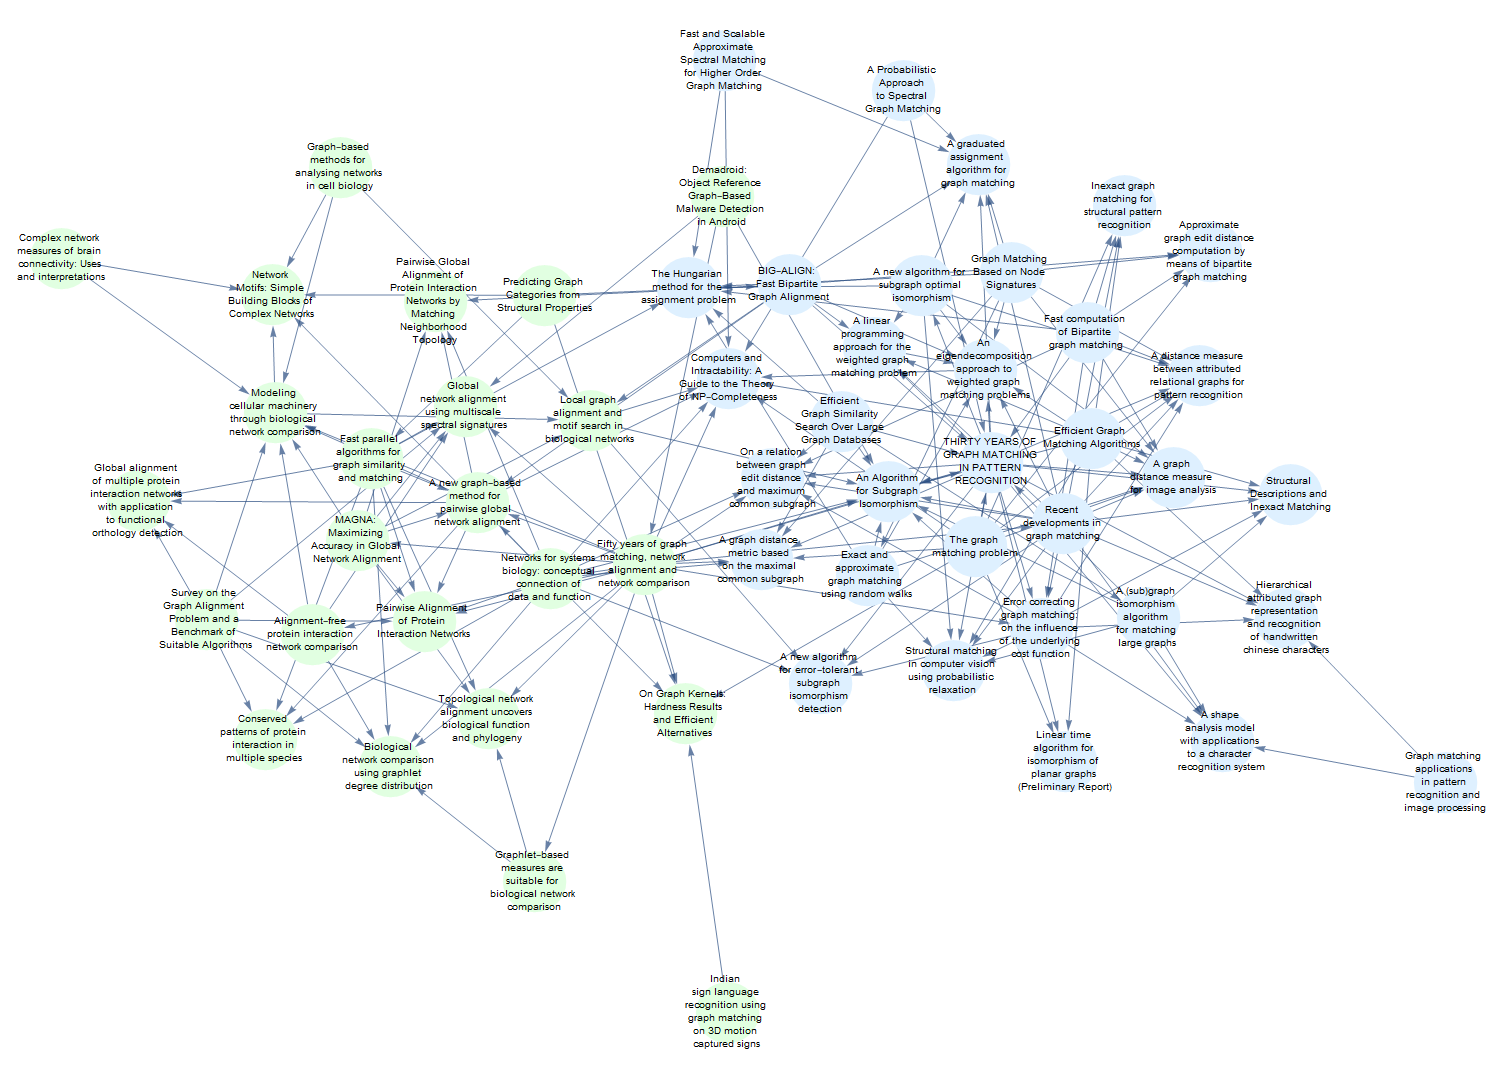
\includegraphics[width=0.9\textwidth]{reading_list0pt9crop.png}
\end{frame}

\begin{frame}{Reading list subnetwork}
\centering
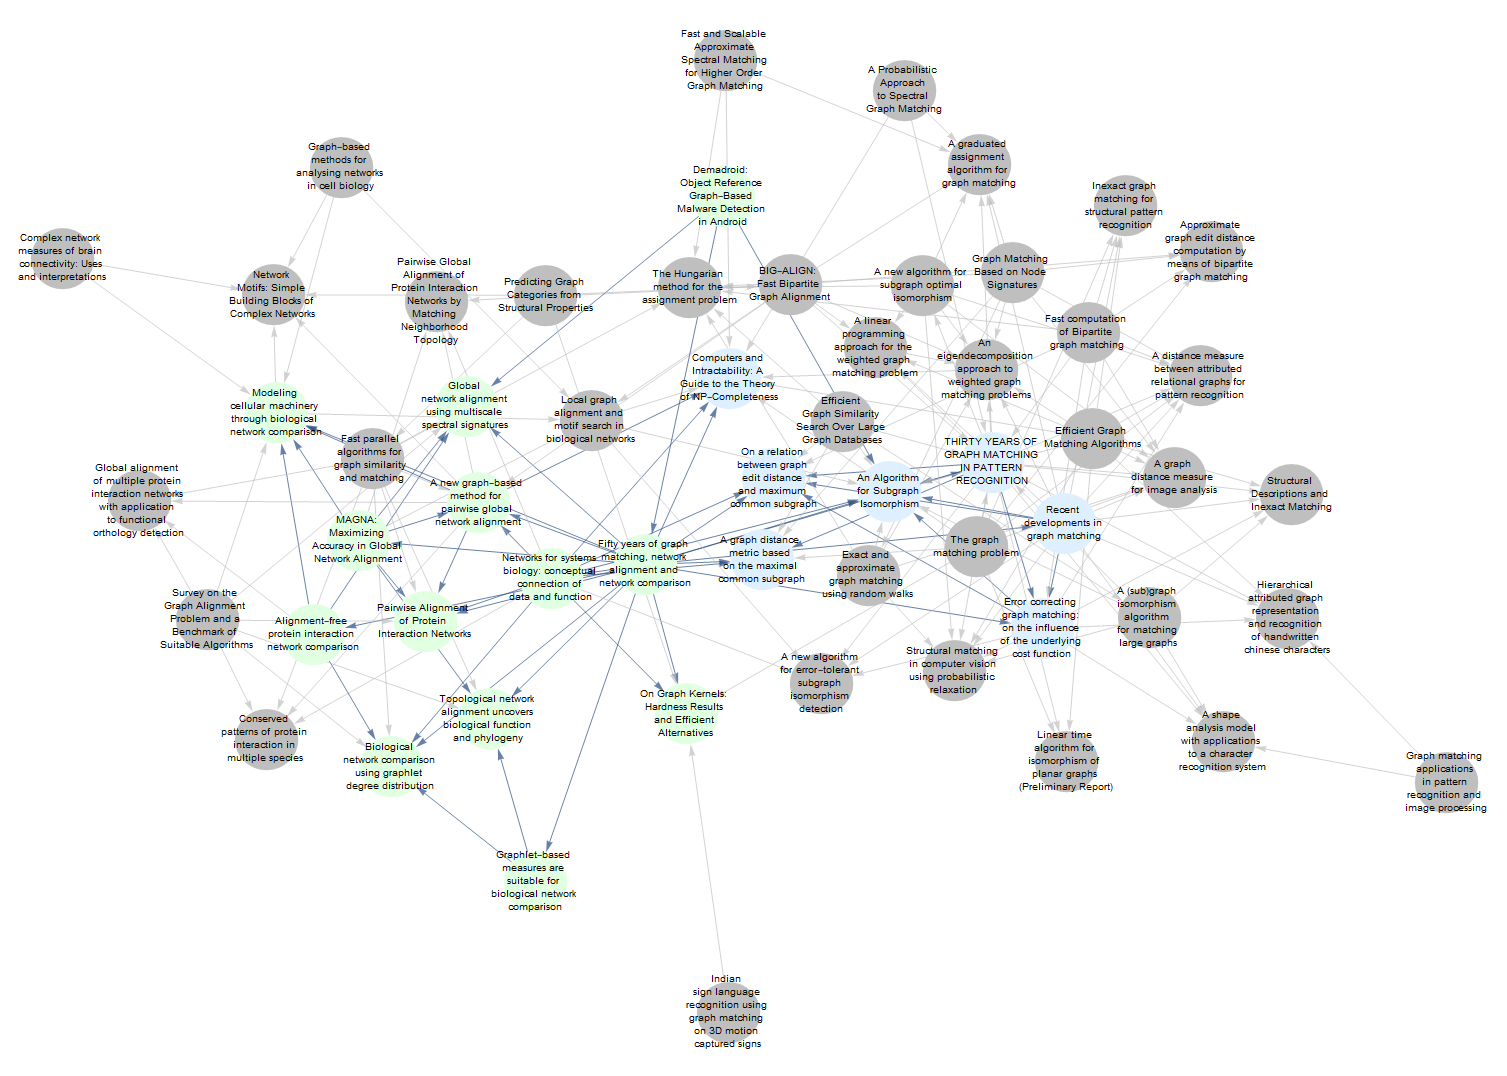
\includegraphics[width=0.9\textwidth]{reading_list_neighborhood0pt9crop.png}
\end{frame}

\begin{frame}{Context}
\begin{itemize}
\item Tabulated metadata (sort by year, title, etc.)
\item Centrality ranks
\item Neighbors within reading list
\item Cocitations
\item Global sense of structure via the partition
\end{itemize}
\pause
Using this context as we read allows us to draw connections and get a better sense of the shape of the field as a whole.
\end{frame}

\begin{frame}{Pattern recognition}
\begin{itemize}
\item Graphs are a powerfully general data structure for the representation of objects and concepts
\pause
\item Particularly useful in computer vision (invariant under positional transformations)
\pause
\begin{itemize}
\item Optical character recognition
\item Biometric identification
\item 3D object recognition
\end{itemize}
\pause
\item Recognition/identification becomes a graph matching problem
\end{itemize}
\end{frame}

\begin{frame}{Graph matching terms}
\begin{itemize}
\item Exact
\item Inexact
\item Error tolerant
\item Optimal
\item Approximate
\item Alignment
\item \sout{Elastic}
\end{itemize}
\end{frame}

\begin{frame}{Exact}
\centering
\scriptsize
\setlength\extrarowheight{3pt}\setlength{\tabcolsep}{3pt}
\begin{tabular}{|L{0.3\linewidth}|C{0.14\linewidth}|C{0.14\linewidth}|C{0.21\linewidth}|}
\hline
 & Graph isomorphism & Subgraph isomorphism & Maximum common induced subgraph \\ \hline\hline
$G_1$ and $G_2$ must have the same number of nodes & X & & \\ \hline
Mapping must include all nodes of either $G_1$ or $G_2$ & X & X & \\ \hline
Mapping must be edge-preserving & X & X & X\hspace{6pt} \\ \hline
NP-complete & Unknown & X & X$^*$ \\ \hline
\end{tabular}
\flushleft\tiny *The associated decision problem of determining whether $G_1$ and $G_2$ have a common induced subgraph with at least $k$ nodes is NP-complete, but the problem of finding the maximum common induced subgraph (as required for graph matching) is NP-hard
\end{frame}

\begin{frame}{Exact}
\centering
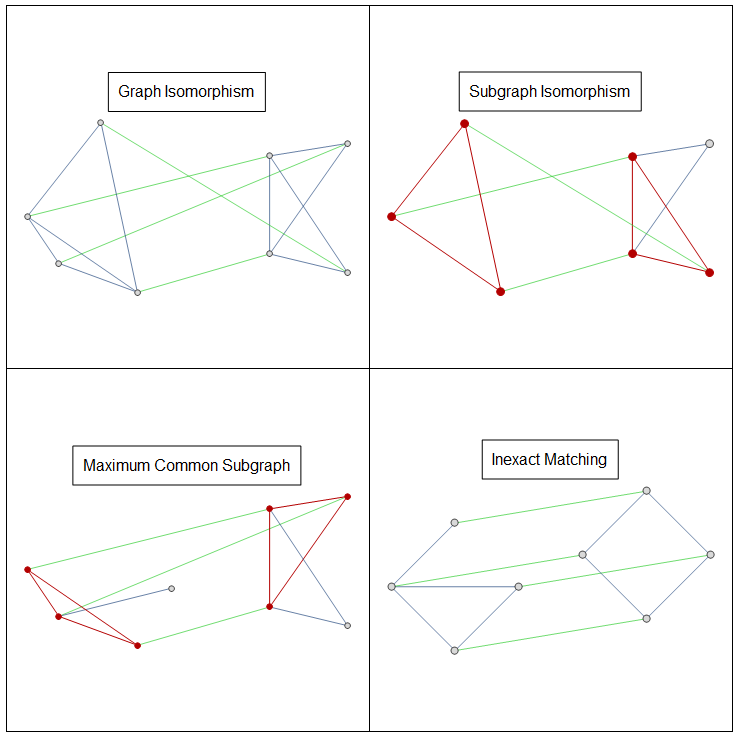
\includegraphics[width=0.65\textwidth]{isomorphism_demos.png}
\end{frame}


\begin{frame}{Comparison of formulations}
\centering
\scriptsize
\setlength\extrarowheight{3pt}\setlength{\tabcolsep}{1pt}
\begin{tabular}{|L{0.16\linewidth}|C{0.19\linewidth}|C{0.11\linewidth}|C{0.195\linewidth}|C{0.105\linewidth}|C{0.165\linewidth}|}
\hline
 & Edge preserving? & Result in? & Mapping seeking? & Optimal? & Complexity \\ \hline\hline
Graph isomorphism & Yes & \{0,1\} & Yes & Yes & Likely between P and NP \\ \hline
Subgraph isomorphism & Yes & \{0,1\} & Yes & Yes & NP-complete \\ \hline
MCS computation & Yes & [0,1] & Yes & Yes & NP-hard \\ \hline
Edit distances (exact) & No & [0,1] & No & Yes & Generally exponential \\ \hline
Edit distances (approximate) & No & [0,1] & No & No & Generally polynomial \\ \hline
Other inexact formulations & No & [0,1] & Sometimes & No* & Generally polynomial \\ \hline
\end{tabular}
\end{frame}


\begin{frame}[fragile]{Search space pruning}

\begin{itemize}
\item Foundational algorithm for subgraph isomorphism is Ullmann 1976
\pause
\item Rules out matching possibilities using two principles
\pause
\begin{itemize}
\item Degree comparison
\item Refinement 
\end{itemize}
\end{itemize}

\pause
\centering
\scriptsize
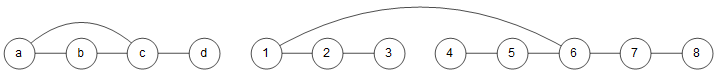
\includegraphics[width=0.8\textwidth]{ullmann_demo_cropped.png} 

\begin{center}
\begin{tikzpicture}
\matrix (m)[
    matrix of math nodes,
    nodes in empty cells,
    inner sep=4pt,
]{ 
 & 1 & 2 & 3 & 4 & 5 & 6 & 7 & 8 \\ \hline
a & 1 & 1 & 0 & 0 & 1 & 1 & 1 & 0 \\
b & 1 & 1 & 0 & 0 & 1 & 1 & 1 & 0 \\
c & 0 & 0 & 0 & 0 & 0 & 1 & 0 & 0 \\
d & 1 & 1 & 1 & 1 & 1 & 1 & 1 & 1 \\
};
\draw (m-5-2.south west) -- (m-1-2.north west);
\end{tikzpicture}
\end{center}

\end{frame}

\begin{frame}[fragile]{Refinement}

\centering
\scriptsize


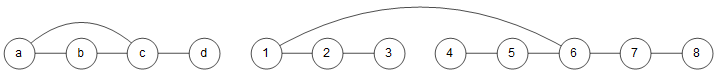
\includegraphics[width=0.8\textwidth]{ullmann_demo_cropped.png} 
\vspace{15pt}

\begin{minipage}{0.35\textwidth}
\begin{center}
\begin{tikzpicture}
\matrix (m)[
    matrix of math nodes,
    nodes in empty cells,
    inner sep=4pt,
]{ 
 & 1 & 2 & 3 & 4 & 5 & 6 & 7 & 8 \\ \hline
a & 1 & 1 & 0 & 0 & 1 & 1 & 1 & 0 \\
b & 1 & 1 & 0 & 0 & 1 & 1 & 1 & 0 \\
c & 0 & 0 & 0 & 0 & 0 & 1 & 0 & 0 \\
d & 1 & 1 & 1 & 1 & 1 & 1 & 1 & 1 \\
};
\fill[gray,opacity=0.2] (m-3-1.south west) rectangle (m-3-9.north east);
\fill[gray,opacity=0.2]  (m-4-1.south west) rectangle (m-4-9.north east);
\fill[gray,opacity=0.2]  (m-5-3.south west) rectangle (m-1-3.north east);
\fill[gray,opacity=0.2]  (m-5-7.south west) rectangle (m-1-7.north east);
\draw (m-5-2.south west) -- (m-1-2.north west);
\draw[black,thick,radius=7pt] (m-2-2) circle;
\draw[green,thick,radius=7pt] (m-3-3) circle;
\draw[green,thick,radius=7pt] (m-4-7) circle;
\end{tikzpicture}
\end{center}
\end{minipage}
\begin{minipage}{0.1\textwidth}
\end{minipage}
\pause
\begin{minipage}{0.35\textwidth}
\begin{center}
\begin{tikzpicture}
\matrix (m)[
    matrix of math nodes,
    nodes in empty cells,
    inner sep=4pt,
]{ 
 & 1 & 2 & 3 & 4 & 5 & 6 & 7 & 8 \\ \hline
a & 1 & \cancel{1} & 0 & 0 & 1 & 1 & 1 & 0 \\
b & 1 & 1 & 0 & 0 & 1 & 1 & 1 & 0 \\
c & 0 & 0 & 0 & 0 & 0 & 1 & 0 & 0 \\
d & 1 & 1 & 1 & 1 & 1 & 1 & 1 & 1 \\
};
\fill[gray,opacity=0.2]  (m-3-1.south west) rectangle (m-3-9.north east);
\fill[gray,opacity=0.2]  (m-4-1.south west) rectangle (m-4-9.north east);
\fill[gray,opacity=0.2]  (m-5-2.south west) rectangle (m-1-2.north east);
\fill[gray,opacity=0.2] (m-5-4.south west) rectangle (m-1-4.north east);
\draw (m-5-2.south west) -- (m-1-2.north west);
\draw[black,thick,radius=7pt] (m-2-3) circle;
\draw[green,thick,radius=7pt] (m-3-2) circle;
\draw[red,thick,radius=7pt] (m-4-2) circle;
\draw[red,thick,radius=7pt] (m-4-4) circle;
\end{tikzpicture}
\end{center}
\end{minipage}

\pause
\begin{center}
\begin{tikzpicture}
\matrix (m)[
    matrix of math nodes,
    nodes in empty cells,
    inner sep=4pt,
]{ 
 & 1 & 2 & 3 & 4 & 5 & 6 & 7 & 8 \\ \hline
a & 1 & 0 & 0 & 0 & 1 & 0 & 1 & 0 \\
b & 1 & 0 & 0 & 0 & 1 & 0 & 1 & 0 \\
c & 0 & 0 & 0 & 0 & 0 & 1 & 0 & 0 \\
d & 1 & 0 & 0 & 0 & 1 & 0 & 1 & 0 \\
};
\draw (m-5-2.south west) -- (m-1-2.north west);
\end{tikzpicture}
\end{center}

\end{frame}

\begin{frame}[fragile]{Backtracking}

\centering
\scriptsize
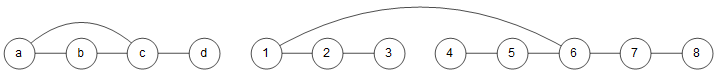
\includegraphics[width=0.8\textwidth]{ullmann_demo_cropped.png} 

\begin{center}
\begin{tikzpicture}
\matrix (m)[
    matrix of math nodes,
    nodes in empty cells,
    inner sep=4pt,
]{ 
 & 1 & 2 & 3 & 4 & 5 & 6 & 7 & 8 \\ \hline
a & \cancel{1} & 0 & 0 & 0 & 1 & 0 & 1 & 0 \\
b & 0 & 0 & 0 & 0 & 1 & 0 & 1 & 0 \\
c & 0 & 0 & 0 & 0 & 0 & 1 & 0 & 0 \\
d & 0 & 0 & 0 & 0 & 1 & 0 & 1 & 0 \\
};
\fill[gray,opacity=0.2]  (m-3-1.south west) rectangle (m-3-9.north east);
\fill[gray,opacity=0.2]  (m-4-1.south west) rectangle (m-4-9.north east);
\fill[gray,opacity=0.2]  (m-5-3.south west) rectangle (m-1-3.north east);
\fill[gray,opacity=0.2] (m-5-7.south west) rectangle (m-1-7.north east);
\draw (m-5-2.south west) -- (m-1-2.north west);
\draw[black,thick,radius=7pt] (m-2-2) circle;
\draw[green,thick,radius=7pt] (m-4-7) circle;
\draw[red,thick,radius=7pt] (m-3-3) circle;
\draw[red,thick,radius=7pt] (m-3-7) circle;
\end{tikzpicture}
\end{center}
\pause

\vspace{-15pt}
\begin{minipage}{0.35\textwidth}
\begin{center}
\begin{tikzpicture}
\matrix (m)[matrix of math nodes,inner sep=4pt
]{ 
 & 1 & 2 & 3 & 4 & 5 & 6 & 7 & 8 \\ \hline
a & 0 & 0 & 0 & 0 & \cancel{1} & 0 & 1 & 0 \\
b & 1 & 0 & 0 & 0 & 0 & 0 & 1 & 0 \\
c & 0 & 0 & 0 & 0 & 0 & 1 & 0 & 0 \\
d & 1 & 0 & 0 & 0 & 0 & 0 & 1 & 0 \\
};
\draw (m-5-2.south west) -- (m-1-2.north west);
\fill[gray,opacity=0.2]  (m-3-1.south west) rectangle (m-3-9.north east);
\fill[gray,opacity=0.2]  (m-4-1.south west) rectangle (m-4-9.north east);
\fill[gray,opacity=0.2]  (m-5-5.south west) rectangle (m-1-5.north east);
\fill[gray,opacity=0.2] (m-5-7.south west) rectangle (m-1-7.north east);
\draw[black,thick,radius=7pt] (m-2-6) circle;
\draw[green,thick,radius=7pt] (m-4-7) circle;
\draw[red,thick,radius=7pt] (m-3-5) circle;
\draw[red,thick,radius=7pt] (m-3-7) circle;
\end{tikzpicture}
\end{center}
\end{minipage}
\begin{minipage}{0.1\textwidth}
\end{minipage}
\pause
\begin{minipage}{0.35\textwidth}
\begin{center}
\begin{tikzpicture}
\matrix (m)[matrix of math nodes,inner sep=4pt
]{ 
 & 1 & 2 & 3 & 4 & 5 & 6 & 7 & 8 \\ \hline
a & 0 & 0 & 0 & 0 & 0 & 0 & \cancel{1} & 0 \\
b & 1 & 0 & 0 & 0 & 1 & 0 & 0 & 0 \\
c & 0 & 0 & 0 & 0 & 0 & 1 & 0 & 0 \\
d & 1 & 0 & 0 & 0 & 1 & 0 & 0 & 0 \\
};
\draw (m-5-2.south west) -- (m-1-2.north west);
\fill[gray,opacity=0.2]  (m-3-1.south west) rectangle (m-3-9.north east);
\fill[gray,opacity=0.2]  (m-4-1.south west) rectangle (m-4-9.north east);
\fill[gray,opacity=0.2]  (m-5-9.south west) rectangle (m-1-9.north east);
\fill[gray,opacity=0.2] (m-5-7.south west) rectangle (m-1-7.north east);
\draw[black,thick,radius=7pt] (m-2-8) circle;
\draw[green,thick,radius=7pt] (m-4-7) circle;
\draw[red,thick,radius=7pt] (m-3-9) circle;
\draw[red,thick,radius=7pt] (m-3-7) circle;
\end{tikzpicture}
\end{center}
\end{minipage}

\end{frame}

\begin{frame}{Edit distances}
\centering
\begin{tabular}{|lcl|l|}
\hline
cat & $\rightarrow$ & ca\textit{r}t & Insertion \\ \hline
\textit{c}art & $\rightarrow$ & \textit{d}art & Substitution \\ \hline
\textit{d}art & $\rightarrow$ & art & Deletion \\ \hline
\textit{ar}t & $\rightarrow$ & \textit{ra}t & Transposition \\ \hline
\end{tabular}
\end{frame}

\begin{frame}{Edit distances}
\centering
\footnotesize
\begin{tabular}{C{0.17\textwidth}C{0.03\textwidth}C{0.17\textwidth}C{0.03\textwidth}C{0.17\textwidth}C{0.03\textwidth}C{0.17\textwidth}}
\multicolumn{3}{c}{Node insertion} & & \multicolumn{3}{c}{Edge insertion} \\
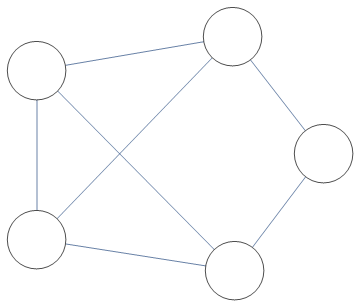
\includegraphics[width=0.17\textwidth]{vertex_insertion_left.png} & $\rightarrow$ & 
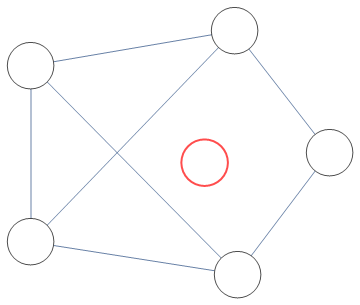
\includegraphics[width=0.17\textwidth]{vertex_insertion_right.png} & & 
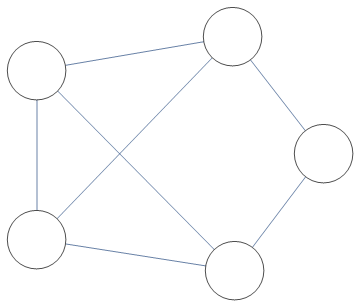
\includegraphics[width=0.17\textwidth]{edge_insertion_left.png} & $\rightarrow$ & 
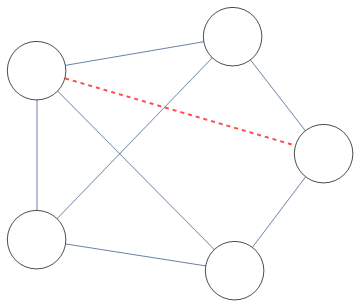
\includegraphics[width=0.17\textwidth]{edge_insertion_right.png} \\
\multicolumn{3}{c}{Node deletion} & &  \multicolumn{3}{c}{Edge deletion} \\
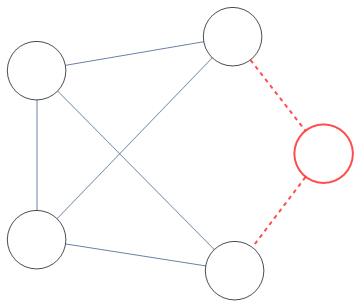
\includegraphics[width=0.17\textwidth]{vertex_deletion_left.png} & $\rightarrow$ & 
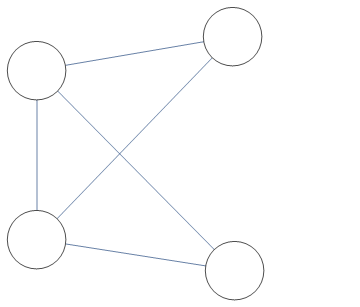
\includegraphics[width=0.17\textwidth]{vertex_deletion_right.png} & & 
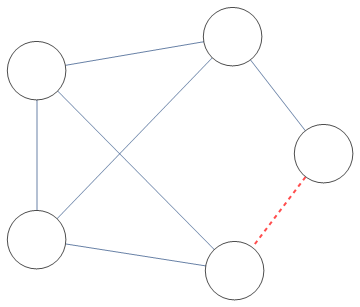
\includegraphics[width=0.17\textwidth]{edge_deletion_left.png} & $\rightarrow$ & 
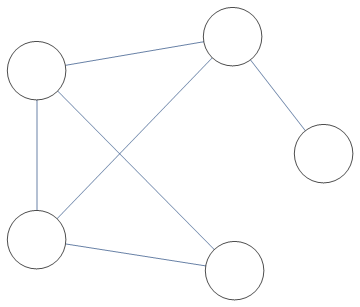
\includegraphics[width=0.17\textwidth]{edge_deletion_right.png} \\
\multicolumn{7}{c}{Node substitution} \\ & & 
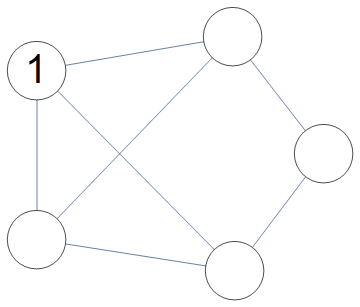
\includegraphics[width=0.17\textwidth]{vertex_substitution_left.png} & $\rightarrow$ &
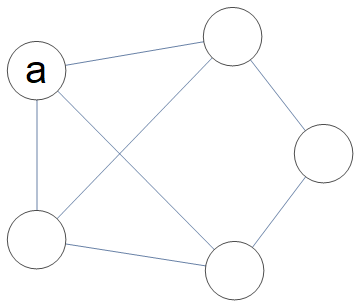
\includegraphics[width=0.17\textwidth]{vertex_substitution_right.png} & & \\
\end{tabular}
\end{frame}

\begin{frame}{Approximate edit distances}
\begin{itemize}
\item We can approximate the graph edit distance using the assignment problem
\pause
\item No longer an optimal method, but can be solved in $O(n^3)$ time by the Hungarian method.
\pause
\end{itemize}
\centering\footnotesize
\begin{tabular}{m{0.3\textwidth}m{0.05\textwidth}m{0.3\textwidth}}
$C = $\bordermatrix{ & 1 & 2 & 3 \cr
a & 3 & 2 & 1 \cr
b & 1 & 3 & 4 \cr
c & 2 & 5 & 2 }
 & $\Leftrightarrow$ &
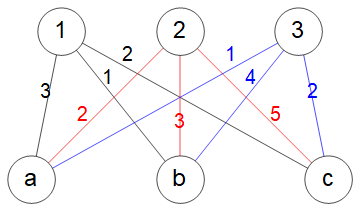
\includegraphics[width=0.3\textwidth]{bipartite_assignment_problem.png} \\
\multicolumn{3}{c}{$A = \{a,b,c\},  B=\{1,2,3\}$}
\end{tabular}
\end{frame}

\begin{frame}{Weighted graph matching problem}
\begin{itemize}
\item Other suboptimal graph matching methods seek to solve the \textit{weighted graph matching problem}.
\pause
\item Instead of indirectly optimizing the quality of a permutation assignment using a cost function, directly minimize $||A_G - PA_HP^T||$ with respect to some norm and permutation matrix $P$, where $A_G$ and $A_H$ are the adjacency matrices of the weighted graphs $G$ and $H$, respectively.
\pause
\item Avoids the heuristics inherent in cost function formulations, but we cannot incorporate external information (important for bio).
\end{itemize}
\end{frame}

\begin{frame}{Biology}
\begin{itemize}
\item Biological network comparison is done primarily on protein-protein interaction (PPI) networks 
\pause
\item Explosion of available PPI data parallels a previous surge of available DNA sequence information
\pause
\item Networks are large, often incompletely explored, non-deterministic, and have real-world meaning
\pause
\item Overall goal is to organize data into models of basic biological processes
\pause
\begin{itemize}
\item Determine function of proteins and groups of interactions
\item Investigate evolutionary relationships across species
\item Develop appropriate random graph models 
\pause
\end{itemize}
\item Different strategies required compared to pattern recognition (small deterministic graphs)
\end{itemize}
\end{frame}


\begin{frame}{Strategies}
\begin{itemize}
\item Count occurrences of very small subgraphs
\begin{itemize}
\item Motifs and graphlets
\item Results in univariate statistics
\item Computational difficulty is in enumerating subgraphs, not matching them
\pause
\end{itemize}
\item Local alignment
\begin{itemize}
\item Find small highly conserved structures
\item Typically searches a deterministically constructed, not necessarily one-to-one mapping
\end{itemize}
\pause
\item Global alignment
\begin{itemize}
\item Find the best comprehensive superimposition of two input networks
\item Typically uses the assignment problem
\end{itemize}
\end{itemize}
\end{frame}

\begin{frame}{Subgraph counting}
\begin{itemize}
\item Graphlets are small connected non-isomorphic induced subgraphs of a simple undirected network
\item Can be used to generalize the degree distribution
\end{itemize}
\centering
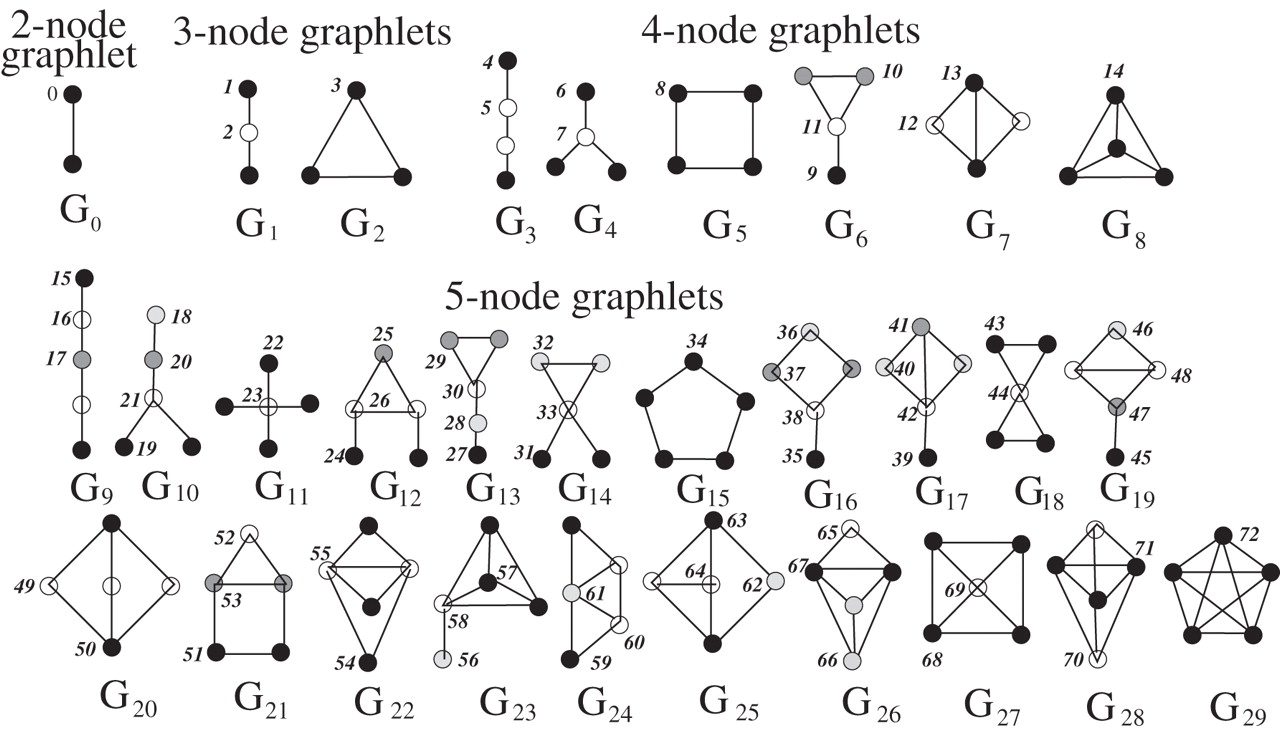
\includegraphics[width=0.8\textwidth]{graphlets_figure.png}

\tiny Figure sourced from ``Biological Network Comparison Using Graphlet Degree Distribution'' (Pr\u{z}ulj, 2007)
\end{frame}

\begin{frame}{Graphlets}
\centering
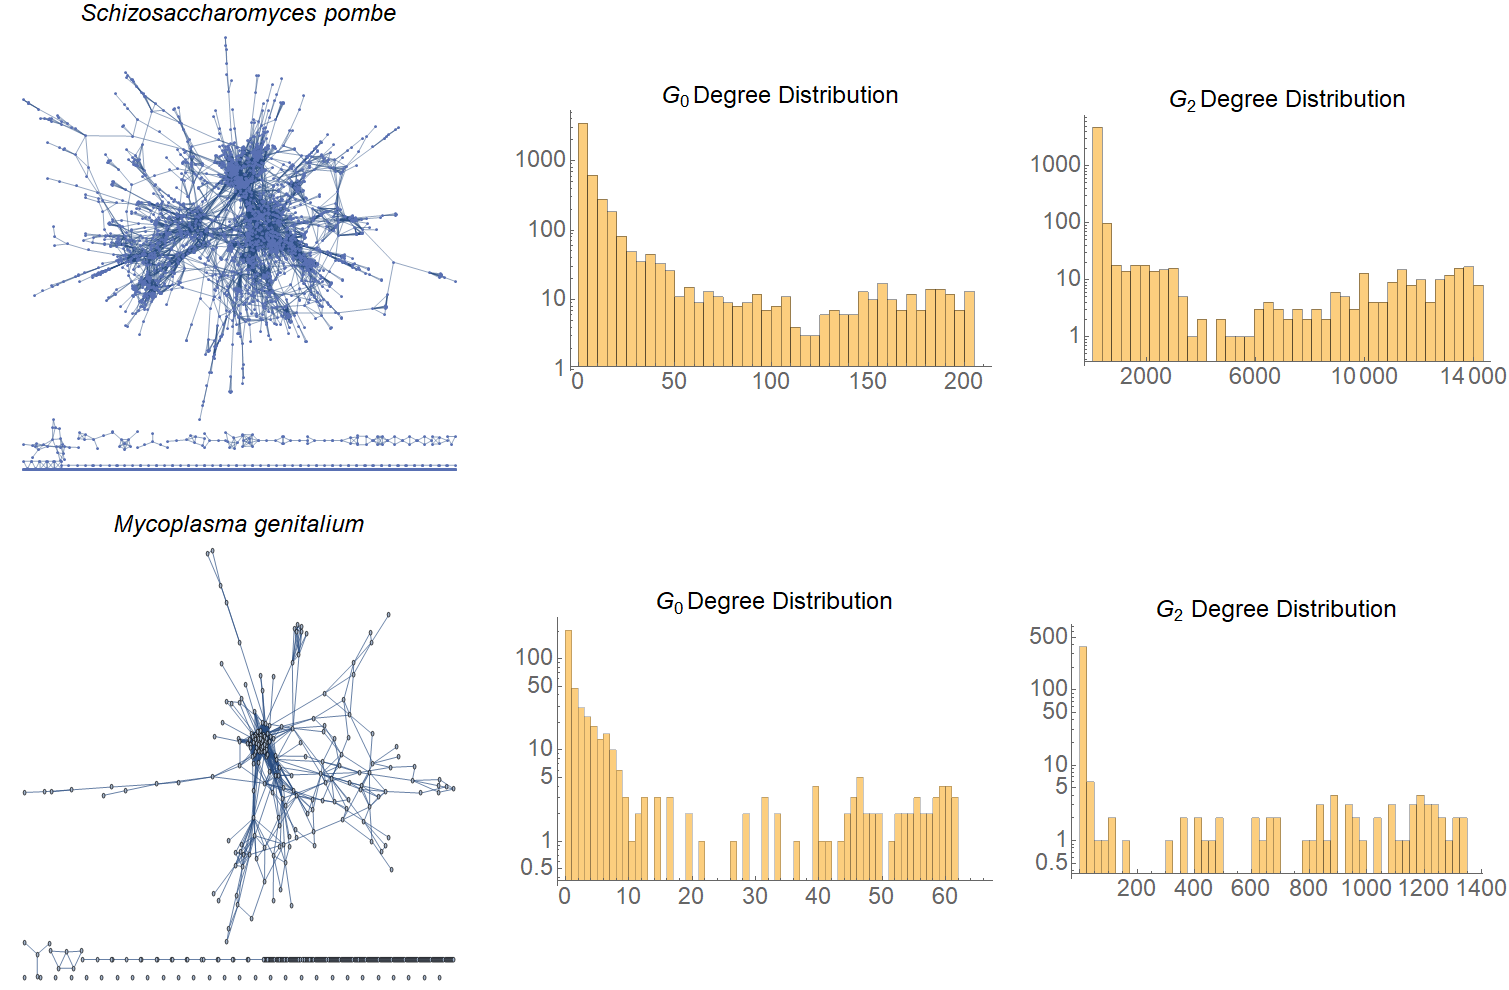
\includegraphics[width=\textwidth]{graphlet_degree_distributions_TOP.png}
\end{frame}

\begin{frame}{Graphlets}
\centering
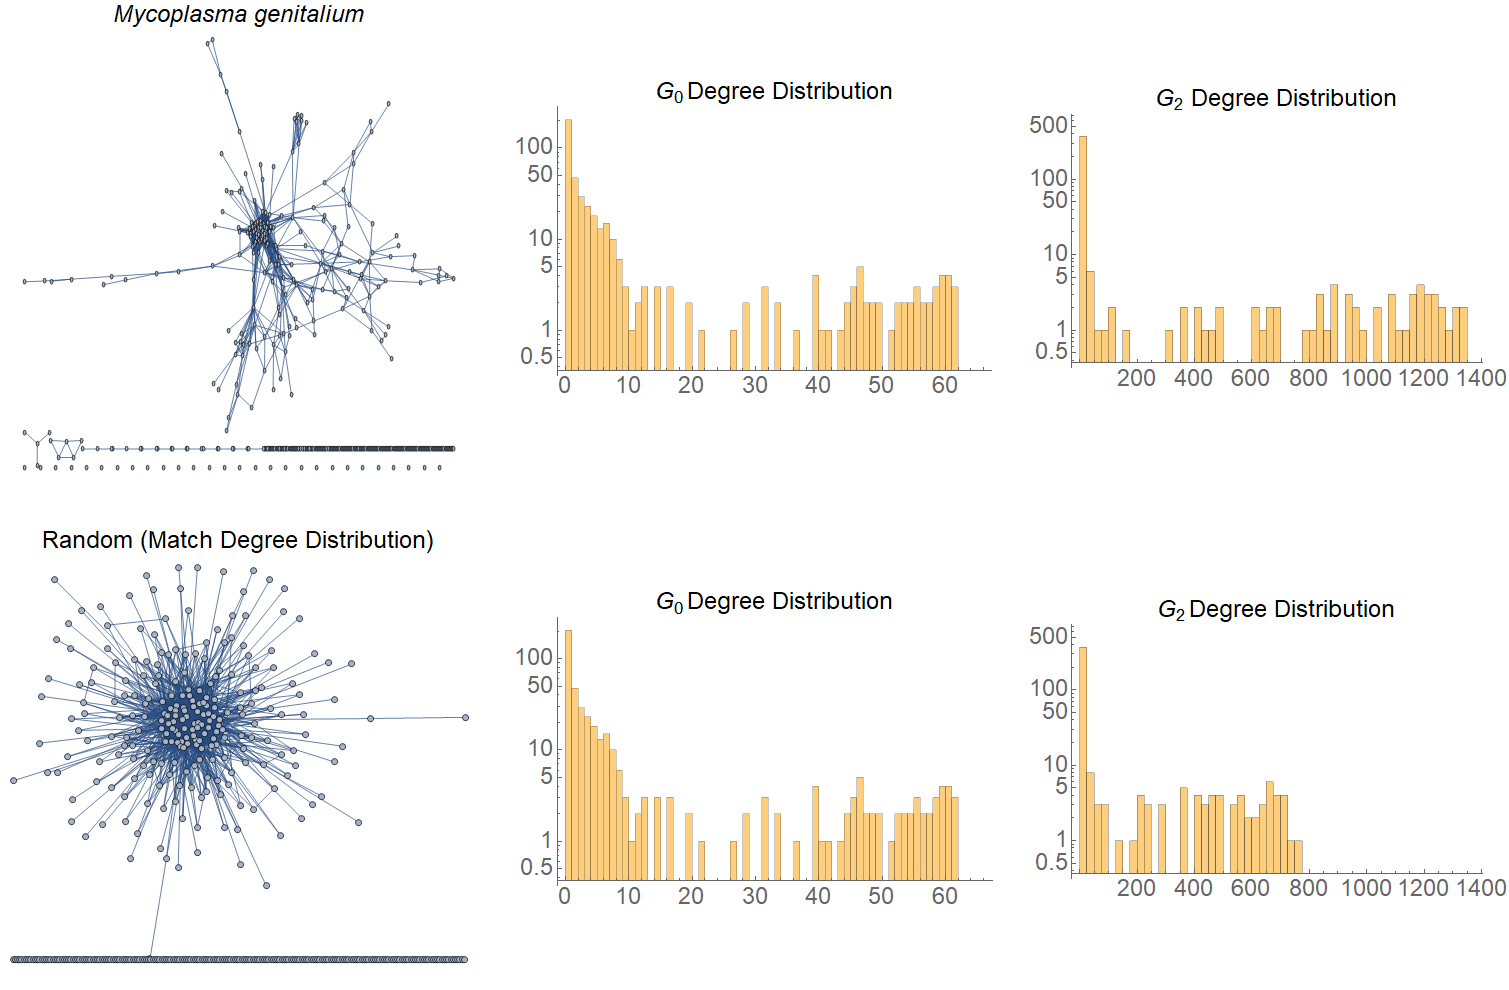
\includegraphics[width=\textwidth]{graphlet_degree_distributions_MIDDLE.png}
\end{frame}

\begin{frame}{Graphlets}
\centering
\footnotesize
{\setlength\extrarowheight{3pt}\setlength{\tabcolsep}{2pt}\setstretch{0.75}
\begin{tabular}{L{0.3\linewidth}C{0.1\linewidth}C{0.1\linewidth}C{0.13\linewidth}C{0.14\linewidth}C{0.14\linewidth}}
\hline
 & Vertices & Edges & Clustering & Maximum $G_0$ degree & Maximum $G_2$ degree \\ \hline

\textit{Mycoplasma genitalium} & 444 & 1860 & 0.758 & 66 & 1376 \\ 
Random (match degree sequence) & 444 & 1860 & 0.420 & 66 & 774  \\ 
Random (match size) & 444 & 1860 &  0.022 & 17 & 6 \\ \hline
\textit{S. pombe} & 5100 & 30118 & 0.757 & 213 & 14592 \\ 
Random (match degree sequence) & 5100 & 30118 & 0.150 & 213 & 3606 \\ 
Random (match size) & 5100 & 30118  & 0.002 & 26 & 3 \\ \hline
\end{tabular}
}
\end{frame}

\begin{frame}{Motifs}
\begin{itemize}
\item Network motifs generalize sequence motifs
\begin{itemize}
\item Find small patterns which are statistically overrepresented compared to a suitable null model
\item Can be directed, unlike graphlets, but do not have multiedges or self loops
\item Dependent on a good random model
\end{itemize}
\end{itemize}
\centering
\begin{minipage}{0.47\linewidth}
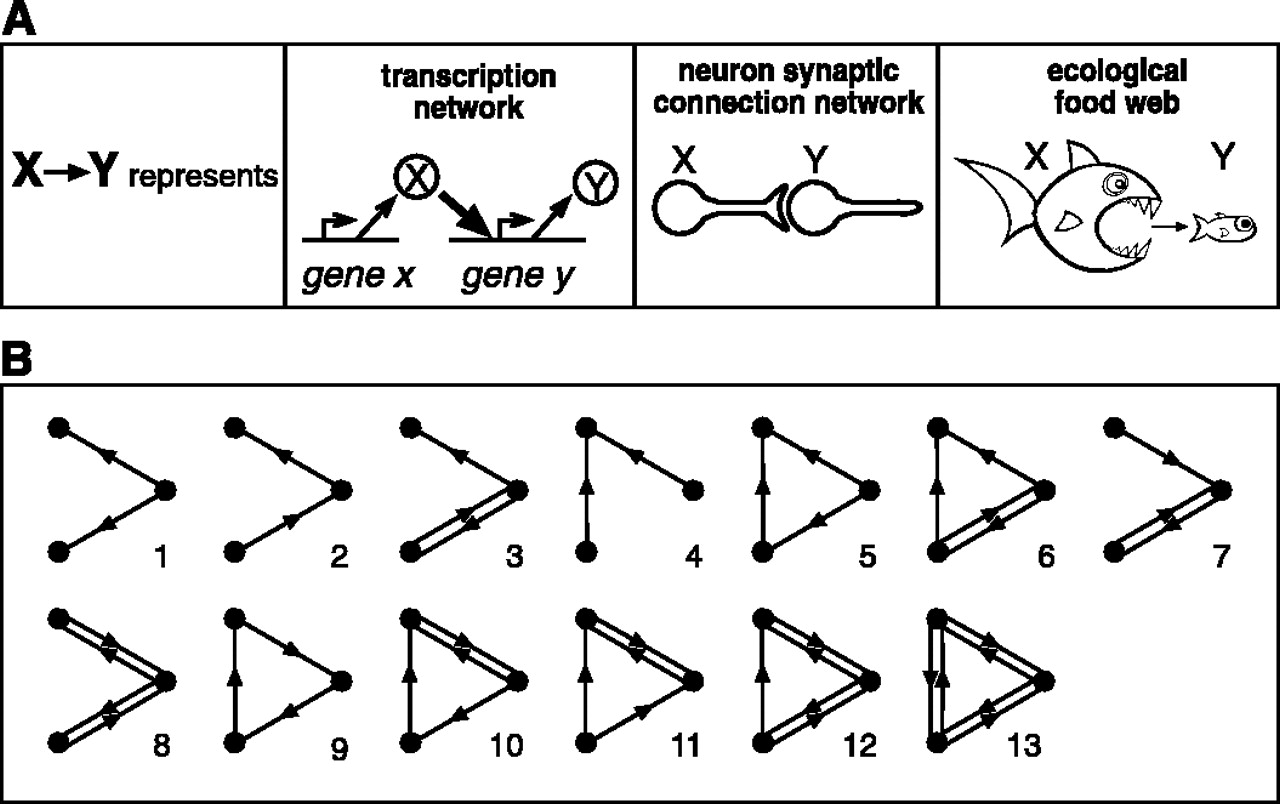
\includegraphics[width=\textwidth]{motif_demo_Milo_2002.png}
\end{minipage}\hfill
\begin{minipage}{0.47\linewidth}
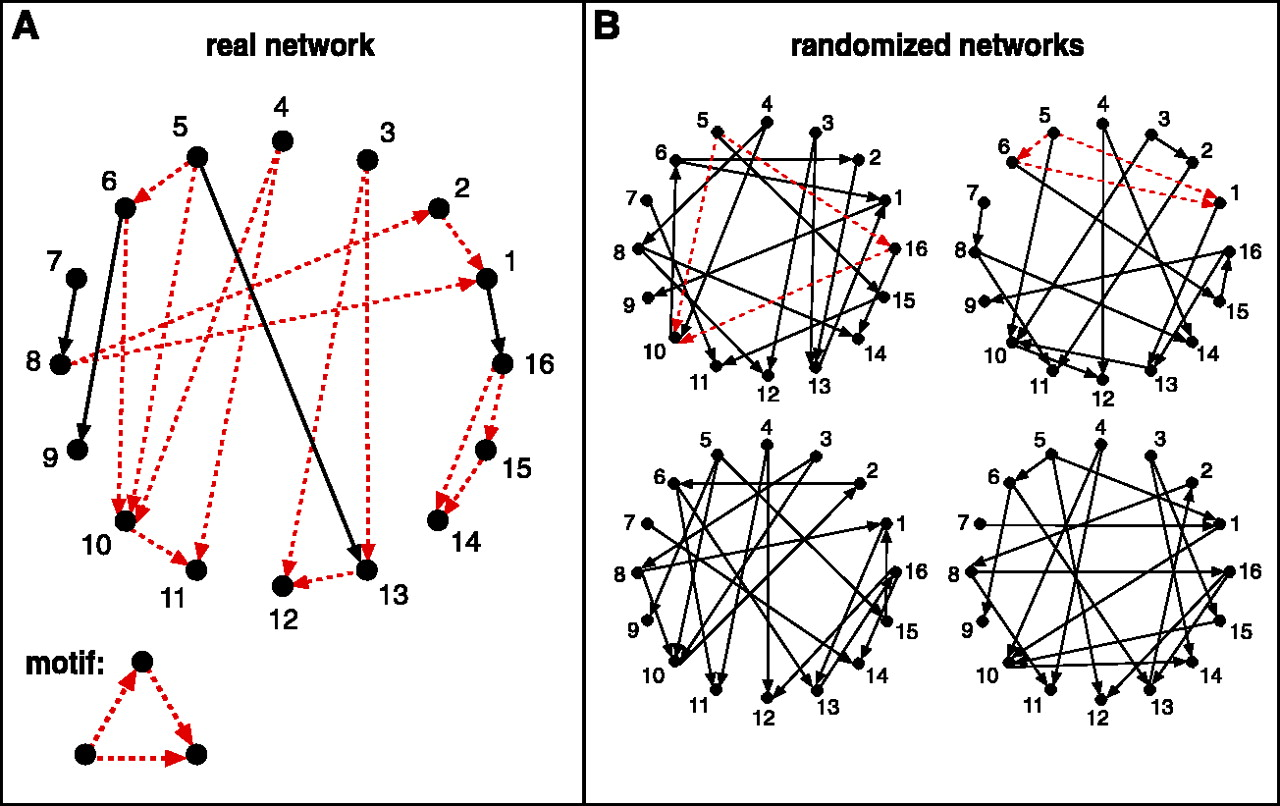
\includegraphics[width=\textwidth]{motif_example_Milo_2002.png}
\end{minipage}
\tiny Figures sourced from ``Network Motifs: Simple Building Blocks of Complex Networks'' (Milo et al., 2002)
\end{frame}

\begin{frame}{Analogy to sequence comparison}
\begin{itemize}
\item The study of biological \textit{networks} has been guided by the study of biological \textit{sequences}
\pause
\item Sequence alignment is based on the assumptions that:
\pause
\begin{enumerate}
\item Patterns which occur frequently are likely to have functional significance
\pause
\item Sequence regions conserved across multiple species are likely to have functional significance
\pause
\item The degree to which sequences differ is related to their evolutionary distance
\end{enumerate}
\pause
\item The study of motifs is based on assumption \#1
\end{itemize}
\end{frame}

\begin{frame}{Alignment}
\begin{itemize}
\item The development of biological network alignment closely parallels that of sequence alignment
\pause
\item Problem
\pause
\begin{itemize}
\item Sequence alignment is $O(mn)$
\item MCS problem is NP-hard
\pause
\item Alignment strategies must compromise
\end{itemize}
\pause
\item Local alignment compromises:
\begin{itemize}
\pause
\item Search for a predetermined pattern 
\item Construct alignment deterministically based on external information
\pause
\end{itemize}
\item Global alignment compromise:
\pause
\begin{itemize}
\item Investigate assignment problem instead of maximum common induced subgraph problem
\end{itemize}
\end{itemize}
\end{frame}

\begin{frame}{Alignment}
\begin{itemize}
\item Local
\begin{itemize}
\item Search for local regions of isomorphism
\item Mappings do not need to be mutually consistent
\end{itemize}
\item Global
\begin{itemize}
\item Single mapping across all parts of the input
\item Large but suboptimally conserved mapped subnetworks
\end{itemize}
\end{itemize}

\begin{minipage}{0.49\linewidth}
\centering
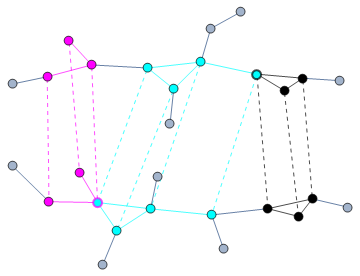
\includegraphics[width=0.75\textwidth]{local_alignment.png}

\footnotesize Local alignment
\end{minipage}\hfill
\begin{minipage}{0.49\linewidth}
\centering
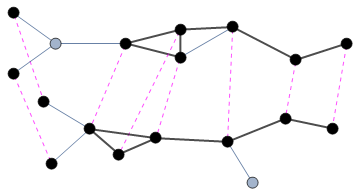
\includegraphics[width=0.75\textwidth]{global_alignment.png}

\footnotesize Global alignment
\end{minipage}
\end{frame}

\begin{frame}{Local alignment}
\begin{itemize}
\item PathBLAST (2004)
\item NetworkBLAST (2008)
\item Graemlin (2006)
\item MAWISH (2006)
\end{itemize}
\centering
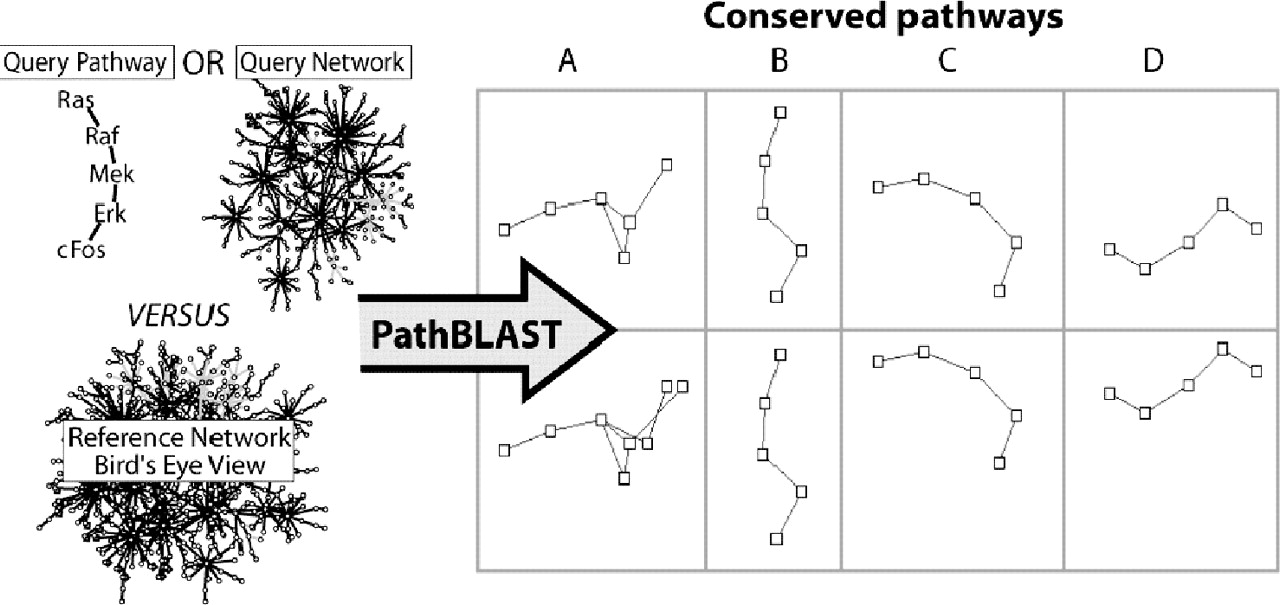
\includegraphics[width=0.75\textwidth]{PathBLAST_demo.png}

\tiny Figure sourced from ``PathBLAST: A Tool For Alignment of Protein Interaction Networks'' (Kelley et al.,2004)
\end{frame}


\begin{frame}{Local alignment}
\centering
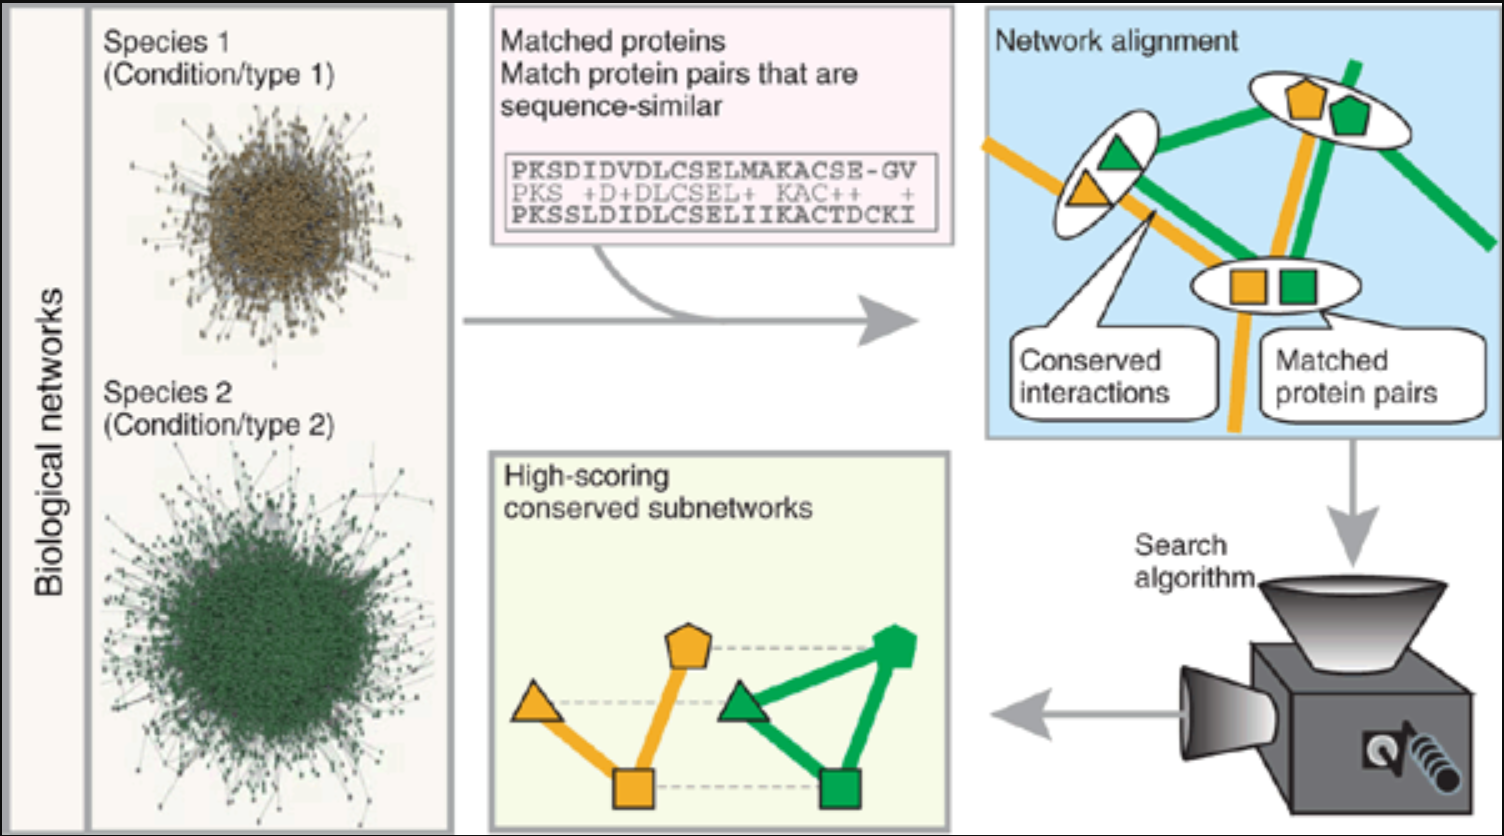
\includegraphics[width=\textwidth]{deterministic_local_alignment.png}
\tiny Figure sourced from ``Modeling cellular machinery through biological network comparison'' (Sharan and Ideker, 2006)
\end{frame}

\begin{frame}{Global alignment}
\begin{itemize}
\item Formulate as the assignment problem
\pause
\item Two steps
\begin{itemize}
\item Cost matrix
\item Construct mapping
\end{itemize}
\pause
\item How does biology's use of the assignment problem differ from pattern recognition?
\pause
\begin{itemize}
\item External node info as well as topological
\item Various measures of alignment quality
\item Neighborhood-based mapping construction
\item Far more common
\end{itemize}
\end{itemize}
\end{frame}

\begin{frame}{Global alignment algorithms discussed}
\begin{itemize}
\item Biology
\begin{itemize}
\item IsoRank (2007) 
\item Natalie (2009) 
\item GRAAL (2010)
\item PINALOG (2012)
\item GHOST (2012)
\item SPINAL (2013)
\item NETAL (2013)
\item MAGNA (2014)
\end{itemize}
\item Non-biology
\begin{itemize}
\item Node signatures (2009)
\item GED approximation (2009)
\item Modified GED approximation (2014)
\end{itemize}
\end{itemize}
\end{frame}

\begin{frame}{IsoRank intuition}
\centering
\footnotesize
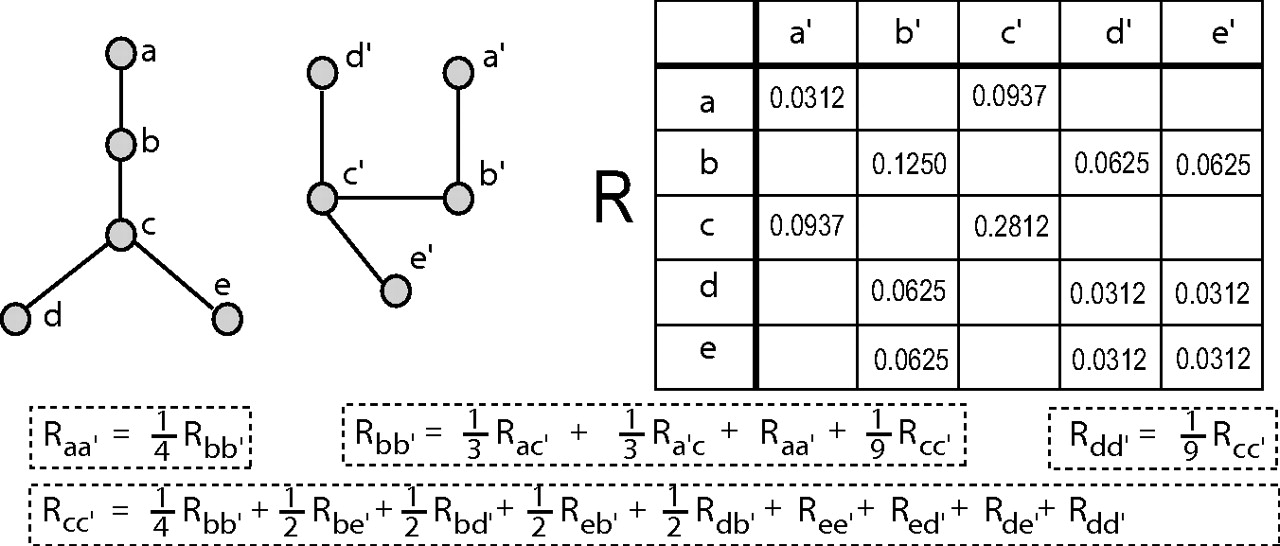
\includegraphics[width=0.9\textwidth]{IsoRank_demo.png}

\tiny Figure sourced from ``Global alignment of multiple protein interaction networks with application to functional orthology detection'' (Singh et al., 2008)


\[R_{ij} = \sum_{u\in N(i)} \sum_{v\in N(j)} \frac{R_{uv}}{|N(u)||N(v)|}, \text{    } i\in V_1, j\in V_2, \]
\end{frame}

\begin{frame}{Conclusion}
\centering
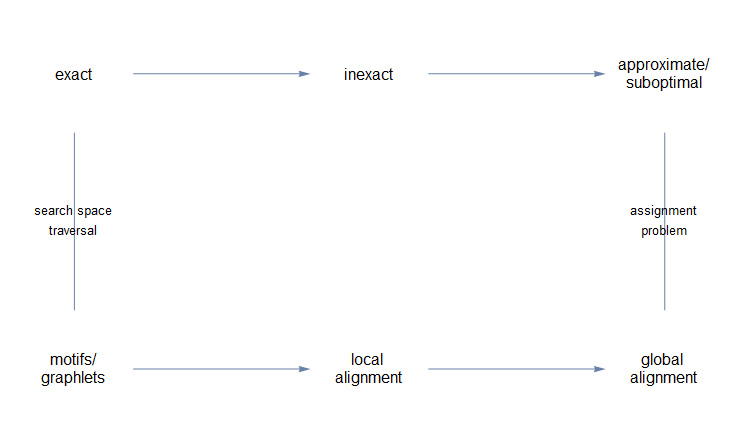
\includegraphics[width=0.9\textwidth]{connections_figure.png}
\end{frame}

\begin{frame}{Conclusion}
\begin{itemize}
\item Networks being investigated inform approach used
\pause
\item Potential cross-applications
\begin{itemize}
\item Graphlets for pattern recognition/database search
\item Global alignment techniques for assignment problem
\item Biological strategies for social networks
\end{itemize}
\pause
\item Utility of citation network method
\end{itemize}
\end{frame}

\begin{frame}
\centering
\Large 
Questions?
\end{frame}

\end{document}